% answers.tex —— 2009 年·普通高等学校招生考试·山东卷·理科 · 参考答案与详细解析片段
% 由 tools/generate_projects.py 依来源总账自 2009/2009_数学真题_山东理_试题.md + 2009/2009_数学真题_山东理_解析正文.md + 2009/2009_数学真题_山东理_答案要点.md 生成，勿手改（改源 MD 后重跑）


\begin{gktip}
固定候选 PDF 仅含题面，无答案、解析和评分标准，原卷亦未标分值；以下为非官方编者独立推导，官方答案字段为空。题面文字层只作定位，分数、根号、上下标与六幅图均以 600 dpi 原页复核。
\end{gktip}

\begin{answer}
\gksolhead{1}{}

\textbf{题目}：

集合 $A=\{0,2,a\}$，$B=\{1,a^2\}$．若 $A\cup B=\{0,1,2,4,16\}$，则 $a$ 的值为（　）

（A）$0$

（B）$1$

（C）$2$

（D）$4$

\Needspace{4\baselineskip}
\textbf{解析}

由 $A\cup B=\{0,1,2,a,a^2\}=\{0,1,2,4,16\}$ 得 $\{a,a^2\}=\{4,16\}$。

若 $a=4$，则 $a^2=16$，并集为 $\{0,1,2,4,16\}$，符合；若 $a=16$，则 $a^2=256$，并集含 $256$，不合。故 $a=4$，选 D。

\gkanswer{答案：D。}

\end{answer}
\begin{answer}
\gksolhead{2}{}

\textbf{题目}：

复数 $\dfrac{3-\mathrm i}{1-\mathrm i}$ 等于（　）

（A）$1+2\mathrm i$

（B）$1-2\mathrm i$

（C）$2+\mathrm i$

（D）$2-\mathrm i$

\Needspace{4\baselineskip}
\textbf{解析}

\nopagebreak[4]
\[\frac{3-\mathrm i}{1-\mathrm i}
=\frac{(3-\mathrm i)(1+\mathrm i)}{(1-\mathrm i)(1+\mathrm i)}
=\frac{3+3\mathrm i-\mathrm i-\mathrm i^2}{2}
=\frac{4+2\mathrm i}{2}=2+\mathrm i,\]

选 C。

\gkanswer{答案：C。}

\end{answer}
\begin{answer}
\gksolhead{3}{}

\textbf{题目}：

将函数 $y=\sin2x$ 的图象向左平移 $\dfrac{\pi}{4}$ 个单位，再向上平移 $1$ 个单位，所得图象的函数解析式是（　）

（A）$y=\cos2x$

（B）$y=2\cos^2x$

（C）$y=1+\sin\left(2x+\dfrac{\pi}{4}\right)$

（D）$y=2\sin^2x$

\Needspace{4\baselineskip}
\textbf{解析}

\Needspace{5\baselineskip}
向左平移 $\frac\pi4$：

\nopagebreak[4]
\[y=\sin2\left(x+\frac\pi4\right)=\sin\left(2x+\frac\pi2\right)=\cos2x,\]

\Needspace{5\baselineskip}
再向上平移 $1$：

\nopagebreak[4]
\[y=1+\cos2x=2\cos^2x,\]

选 B。

\gkanswer{答案：B。}

\end{answer}
\begin{answer}
\gksolhead{4}{}

\textbf{题目}：

一空间几何体的三视图如图所示，则该几何体的体积为（　）

（A）$2\pi+2\sqrt3$

（B）$4\pi+2\sqrt3$

（C）$2\pi+\dfrac{2\sqrt3}{3}$

（D）$4\pi+\dfrac{2\sqrt3}{3}$
\nopagebreak[4]
\begin{center}% 2009 年山东卷理科第 4 题：三视图（圆柱与其上四棱锥）。
% 来源 PDF：普通高考/2009/2009山东理.pdf，SHA256 6c3546f276b37d6ff4fa1a8cdf77e8356b8a4c0e713e9e5485bb47fcd5ed660f
% 原页：第 1 页（A3 三栏）第 1 栏中部，印刷页 545。
% 重绘依据：正视图为 2×2 矩形上方接顶角三角形（斜棱标 2），侧视图同形；
%   俯视图为半径 1 的圆内接正方形（对角线为两条互相垂直的直径）；尺寸按原图标注。
\begin{tikzpicture}[scale=0.8, semithick, every node/.style={inner sep=1.3pt, font=\small}]
  % 正视图
  \begin{scope}[shift={(0,0)}]
    \draw (0,0) rectangle (2,2);
    \draw (0,2) -- (1,3.0) -- (2,2);
    \node[anchor=east] at (-0.12,1) {$2$};
    \node[anchor=north] at (1,-0.12) {$2$};
    \node[anchor=south east] at (0.42,2.55) {$2$};
    \node[anchor=north] at (1,-0.42) {正（主）视图};
  \end{scope}
  % 侧视图
  \begin{scope}[shift={(4.2,0)}]
    \draw (0,0) rectangle (2,2);
    \draw (0,2) -- (1,3.0) -- (2,2);
    \node[anchor=north] at (1,-0.12) {$2$};
    \node[anchor=south east] at (0.42,2.55) {$2$};
    \node[anchor=north] at (1,-0.42) {侧（左）视图};
  \end{scope}
  % 俯视图
  \begin{scope}[shift={(1.0,-4.6)}]
    \draw (1,1) circle (1);
    \draw (0,1) -- (2,1) -- (1,2) -- (1,0) -- cycle;
    \node[anchor=north] at (1,-0.18) {俯视图};
  \end{scope}
\end{tikzpicture}
\end{center}
\nopagebreak[4]
\Needspace{4\baselineskip}
\textbf{解析}

由三视图：下部为底面半径 $1$、高 $2$ 的圆柱；上部为四棱锥，底面是圆柱底面的内接正方形（俯视图中圆内接正方形，对角线为两条互相垂直的直径，长 $2$），侧棱长 $2$。

\Needspace{5\baselineskip}
圆柱体积

\nopagebreak[4]
\[V_1=\pi\cdot1^2\cdot2=2\pi .\]

\Needspace{5\baselineskip}
内接正方形对角线 $2$，边长 $\sqrt2$，中心到顶点距离 $1$，故四棱锥高

\nopagebreak[4]
\[h=\sqrt{2^2-1^2}=\sqrt3,\]

\nopagebreak[4]
\[V_2=\frac13\cdot(\sqrt2)^2\cdot\sqrt3=\frac{2\sqrt3}{3}.\]

\nopagebreak[4]
\[V=V_1+V_2=2\pi+\frac{2\sqrt3}{3},\]

选 C。

\gkanswer{答案：C。}

\end{answer}
\begin{answer}
\gksolhead{5}{}

\textbf{题目}：

已知 $\alpha,\beta$ 表示两个不同的平面，$m$ 为平面 $\alpha$ 内的一条直线，则「$\alpha\perp\beta$」是「$m\perp\beta$」的（　）

（A）充分不必要条件

（B）必要不充分条件

（C）充要条件

（D）既不充分也不必要条件

\Needspace{4\baselineskip}
\textbf{解析}

若 $m\perp\beta$ 且 $m\subset\alpha$，由面面垂直的判定定理得 $\alpha\perp\beta$，故「$\alpha\perp\beta$」是必要条件。

反之，$\alpha\perp\beta$ 时，平面 $\alpha$ 内只有垂直于交线的直线才垂直于 $\beta$；取 $m$ 为 $\alpha$ 内与交线平行的直线，则 $m\parallel\beta$，故不充分。

选 B。

\gkanswer{答案：B。}

\end{answer}
\begin{answer}
\gksolhead{6}{}

\textbf{题目}：

函数 $y=\dfrac{\mathrm e^x+\mathrm e^{-x}}{\mathrm e^x-\mathrm e^{-x}}$ 的图象大致为（　）
\nopagebreak[4]
\begin{center}% 2009 年山东卷理科第 6 题：y=(e^x+e^{-x})/(e^x-e^{-x}) 的四个候选图象。
% 来源 PDF：普通高考/2009/2009山东理.pdf，SHA256 6c3546f276b37d6ff4fa1a8cdf77e8356b8a4c0e713e9e5485bb47fcd5ed660f
% 原页：第 1 页（A3 三栏）第 2 栏上部，印刷页 545。
% 重绘依据：(A) 双曲余切：右支由 +∞ 递减趋于 1，左支由 −1 递减到 −∞，虚线为 y=±1；
%   (B) 在 y 轴处有跳跃（(0,1) 与 (0,−1) 为空心点），整体递增；
%   (C) 过原点、以 y 轴为竖直切线、两侧递增（形如 y=x^{1/3}）；
%   (D) 关于 y 轴对称、在原点取 0、两侧递增（形如 y=|x|^{1/3}）。
\begin{tikzpicture}[semithick, every node/.style={inner sep=1.1pt, font=\small}]
  % (A)
  \begin{scope}[shift={(0,0)}, x=0.62cm, y=0.62cm]
    \draw[dashed] (-2.0,1) -- (2.4,1);
    \draw[dashed] (-2.0,-1) -- (2.4,-1);
    \draw[-{Stealth}] (-2.1,0) -- (2.5,0) node[right] {$x$};
    \draw[-{Stealth}] (0,-2.2) -- (0,2.2) node[above] {$y$};
    \begin{scope}
      \clip (-2.1,-2.2) rectangle (2.5,2.2);
      \draw[domain=0.14:2.3,samples=140,smooth,variable=\x]
        plot (\x, {(exp(\x)+exp(-\x))/(exp(\x)-exp(-\x))});
      \draw[domain=-2.3:-0.14,samples=140,smooth,variable=\x]
        plot (\x, {(exp(\x)+exp(-\x))/(exp(\x)-exp(-\x))});
    \end{scope}
    \node[anchor=north] at (0.02,-0.10) {$O$};
    \node[anchor=south east] at (-0.06,1) {$1$};
    \node[anchor=north east] at (-0.06,-1) {$-1$};
    \node at (0.6,-2.85) {(A)};
  \end{scope}
  % (B)
  \begin{scope}[shift={(5.0,0)}, x=0.62cm, y=0.62cm]
    \draw[-{Stealth}] (-2.1,0) -- (2.5,0) node[right] {$x$};
    \draw[-{Stealth}] (0,-2.2) -- (0,2.2) node[above] {$y$};
    \begin{scope}
      \clip (-2.1,-2.2) rectangle (2.5,2.2);
      \draw[domain=-2.2:-0.001,samples=100,smooth,variable=\x]
        plot (\x, {1+0.55*\x+0.10*\x*\x});
      \draw[domain=0.001:2.2,samples=100,smooth,variable=\x]
        plot (\x, {-1+0.55*\x+0.10*\x*\x});
    \end{scope}
    \draw[fill=white] (0,1) circle (1.4pt);
    \draw[fill=white] (0,-1) circle (1.4pt);
    \node[anchor=north] at (0.02,-0.10) {$O$};
    \node[anchor=west] at (0.08,1) {$1$};
    \node at (0.6,-2.85) {(B)};
  \end{scope}
  % (C)
  \begin{scope}[shift={(0,-5.4)}, x=0.62cm, y=0.62cm]
    \draw[-{Stealth}] (-2.1,0) -- (2.5,0) node[right] {$x$};
    \draw[-{Stealth}] (0,-2.2) -- (0,2.2) node[above] {$y$};
    \begin{scope}
      \clip (-2.1,-2.2) rectangle (2.5,2.2);
      \draw[domain=-2.2:2.2,samples=160,smooth,variable=\x]
        plot (\x, {sign(\x)*pow(abs(\x),1/3)*1.25});
    \end{scope}
    \node[anchor=north] at (0.02,-0.10) {$O$};
    \node[anchor=south west] at (1,-0.02) {$1$};
    \node at (0.6,-2.85) {(C)};
  \end{scope}
  % (D)
  \begin{scope}[shift={(5.0,-5.4)}, x=0.62cm, y=0.62cm]
    \draw[-{Stealth}] (-2.1,0) -- (2.5,0) node[right] {$x$};
    \draw[-{Stealth}] (0,-2.2) -- (0,2.2) node[above] {$y$};
    \begin{scope}
      \clip (-2.1,-2.2) rectangle (2.5,2.2);
      \draw[domain=0.001:2.2,samples=100,smooth,variable=\x]
        plot (\x, {pow(\x,1/3)*1.25});
      \draw[domain=-2.2:-0.001,samples=100,smooth,variable=\x]
        plot (\x, {pow(-\x,1/3)*1.25});
    \end{scope}
    \node[anchor=north] at (0.02,-0.10) {$O$};
    \node[anchor=south east] at (-0.05,1.25) {$1$};
    \node at (0.6,-2.85) {(D)};
  \end{scope}
\end{tikzpicture}
\end{center}
\nopagebreak[4]
\Needspace{4\baselineskip}
\textbf{解析}

\nopagebreak[4]
\[f(x)=\frac{\mathrm e^x+\mathrm e^{-x}}{\mathrm e^x-\mathrm e^{-x}},\qquad x\neq0,\]

\nopagebreak[4]
\[f(-x)=\frac{\mathrm e^{-x}+\mathrm e^{x}}{\mathrm e^{-x}-\mathrm e^{x}}=-f(x),\]

为奇函数。

$x>0$ 时分子分母同除以 $\mathrm e^x$：$f(x)=\dfrac{1+\mathrm e^{-2x}}{1-\mathrm e^{-2x}}$，随 $x$ 增大而减小，$x\to0^+$ 时 $f\to+\infty$，$x\to+\infty$ 时 $f\to1$。由奇对称，$x<0$ 时 $f<-1$、递减，$x\to-\infty$ 时 $f\to-1$。

故图象以 $y$ 轴为竖直渐近线、以 $y=\pm1$ 为水平渐近线，选 A。

\gkanswer{答案：A。}

\end{answer}
\begin{answer}
\gksolhead{7}{}

\textbf{题目}：

设 $P$ 是 $\triangle ABC$ 所在平面内的一点，$\overrightarrow{BC}+\overrightarrow{BA}=2\overrightarrow{BP}$，则（　）

（A）$\overrightarrow{PA}+\overrightarrow{PB}=\mathbf 0$

（B）$\overrightarrow{PC}+\overrightarrow{PA}=\mathbf 0$

（C）$\overrightarrow{PB}+\overrightarrow{PC}=\mathbf 0$

（D）$\overrightarrow{PA}+\overrightarrow{PB}+\overrightarrow{PC}=\mathbf 0$

\Needspace{4\baselineskip}
\textbf{解析}

\Needspace{5\baselineskip}
由

\nopagebreak[4]
\[\overrightarrow{BC}+\overrightarrow{BA}=2\overrightarrow{BP}\]

\Needspace{5\baselineskip}
得 $\overrightarrow{BP}=\dfrac{\overrightarrow{BA}+\overrightarrow{BC}}{2}$，即 $P$ 是 $AC$ 的中点。于是

\nopagebreak[4]
\[\overrightarrow{PC}+\overrightarrow{PA}=\mathbf 0,\]

选 B。

\gkanswer{答案：B。}

\end{answer}
\begin{answer}
\gksolhead{8}{}

\textbf{题目}：

某工厂对一批产品进行了抽样检测．如图是根据抽样检测后的产品净重（单位：克）数据绘制的频率分布直方图，其中产品净重的范围是 $[96,106]$，样本数据分组为 $[96,98)$，$[98,100)$，$[100,102)$，$[102,104)$，$[104,106]$，已知样本中产品净重小于 $100$ 克的个数是 $36$，则样本中净重大于或等于 $98$ 克并且小于 $104$ 克的产品的个数是（　）

（A）$90$

（B）$75$

（C）$60$

（D）$45$
\nopagebreak[4]
\begin{center}% 2009 年山东卷理科第 8 题：产品净重的频率分布直方图。
% 来源 PDF：普通高考/2009/2009山东理.pdf，SHA256 6c3546f276b37d6ff4fa1a8cdf77e8356b8a4c0e713e9e5485bb47fcd5ed660f
% 原页：第 1 页（A3 三栏）第 2 栏中下部，印刷页 545。
% 重绘依据：横轴为净重（克），标 96、98、100、102、104、106；纵轴为「频率/组距」，
%   刻度 0.050、0.075、0.100、0.125、0.150；五根矩形的高度依次为
%   0.050、0.100、0.150、0.125、0.075（组距 2），虚线标出各高度。
\begin{tikzpicture}[scale=0.9, semithick, every node/.style={inner sep=1.2pt, font=\small}]
  % 坐标轴
  \draw[-{Stealth}] (0,0) -- (7.95,0) node[right] {克};
  \draw[-{Stealth}] (0,0) -- (0,4.6) node[above] {频率/组距};
  % 纵轴刻度与虚线
  \foreach \y/\lab in {1/0.050, 1.5/0.075, 2/0.100, 2.5/0.125, 3/0.150} {
    \node[anchor=east] at (-0.08,\y) {\lab};
    \draw[densely dashed] (0,\y) -- (7.2,\y);
  }
  % 五根矩形：区间宽 1.4，依次从 x=0.2 起
  \foreach \i/\h in {0/1, 1/2, 2/3, 3/2.5, 4/1.5} {
    \pgfmathsetmacro{\x}{\i*1.4+0.2}
    \draw (\x,0) rectangle (\x+1.4,\h);
  }
  % 横轴刻度
  \foreach \i/\lab in {0/96, 1/98, 2/100, 3/102, 4/104, 5/106} {
    \pgfmathsetmacro{\x}{\i*1.4+0.2}
    \draw (\x,0) -- (\x,-0.08);
    \node[anchor=north] at (\x,-0.08) {\lab};
  }
\end{tikzpicture}
\end{center}
\nopagebreak[4]
\Needspace{4\baselineskip}
\textbf{解析}

\Needspace{5\baselineskip}
各组频率（频率 $=$ 纵坐标 $\times$ 组距 $2$）：

\nopagebreak[4]
\[0.050\times2=0.1,\quad 0.100\times2=0.2,\quad 0.150\times2=0.3,\]
\nopagebreak[4]
\[0.125\times2=0.25,\quad 0.075\times2=0.15 .\]

\Needspace{5\baselineskip}
净重小于 $100$ 克的频率为 $0.1+0.2=0.3$，故样本容量

\nopagebreak[4]
\[N=\frac{36}{0.3}=120 .\]

\Needspace{5\baselineskip}
净重大于或等于 $98$ 克且小于 $104$ 克的频率为

\nopagebreak[4]
\[0.2+0.3+0.25=0.75,\]

\Needspace{5\baselineskip}
个数为

\nopagebreak[4]
\[120\times0.75=90,\]

选 A。

\gkanswer{答案：A。}

\end{answer}
\begin{answer}
\gksolhead{9}{}

\textbf{题目}：

设双曲线 $\dfrac{x^2}{a^2}-\dfrac{y^2}{b^2}=1$ 的一条渐近线与抛物线 $y=x^2+1$ 只有一个公共点，则双曲线的离心率为（　）

（A）$\frac54$

（B）$5$

（C）$\frac{\sqrt5}{2}$

（D）$\sqrt5$

\Needspace{4\baselineskip}
\textbf{解析}

\Needspace{5\baselineskip}
渐近线 $y=\pm\dfrac ba x$，取 $y=\dfrac ba x$。与 $y=x^2+1$ 联立：

\nopagebreak[4]
\[x^2-\frac ba x+1=0 .\]

\Needspace{5\baselineskip}
只有一个公共点即判别式为零：

\nopagebreak[4]
\[\frac{b^2}{a^2}-4=0\ \Longrightarrow\ \frac ba=2 .\]

\Needspace{5\baselineskip}
故

\nopagebreak[4]
\[e=\sqrt{1+\frac{b^2}{a^2}}=\sqrt5,\]

选 D。

\gkanswer{答案：D。}

\end{answer}
\begin{answer}
\gksolhead{10}{}

\textbf{题目}：

定义在 $\mathbf R$ 上的函数 $f(x)$ 满足 $f(x)=\begin{cases}\log_2(1-x),&x\leqslant0,\\ f(x-1)-f(x-2),&x>0,\end{cases}$ 则 $f(2009)$ 的值为（　）

（A）$-1$

（B）$0$

（C）$1$

（D）$2$

\Needspace{4\baselineskip}
\textbf{解析}

\Needspace{5\baselineskip}
由 $f(x)=f(x-1)-f(x-2)$ 取 $x+2$：

\nopagebreak[4]
\[f(x+2)=f(x+1)-f(x),\]

\Needspace{5\baselineskip}
再取 $x+1$：$f(x+3)=f(x+2)-f(x+1)=-f(x)$，故

\nopagebreak[4]
\[f(x+6)=-f(x+3)=f(x),\]

\Needspace{5\baselineskip}
即 $6$ 为周期。$2009=6\times334+5$，故 $f(2009)=f(5)$。

\nopagebreak[4]
\[f(0)=\log_2 1=0,\qquad f(-1)=\log_2 2=1,\]

\nopagebreak[4]
\[f(1)=f(0)-f(-1)=-1,\qquad f(2)=f(1)-f(0)=-1,\]

\nopagebreak[4]
\[f(3)=f(2)-f(1)=0,\qquad f(4)=f(3)-f(2)=1,\]

\nopagebreak[4]
\[f(5)=f(4)-f(3)=1,\]

选 C。

\gkanswer{答案：C。}

\end{answer}
\begin{answer}
\gksolhead{11}{}

\textbf{题目}：

在区间 $[-1,1]$ 上随机取一个数 $x$，$\cos\dfrac{\pi x}{2}$ 的值介于 $0$ 到 $\dfrac12$ 之间的概率为（　）

（A）$\frac13$

（B）$\frac2\pi$

（C）$\frac12$

（D）$\frac23$

\Needspace{4\baselineskip}
\textbf{解析}

\Needspace{5\baselineskip}
$x\in[-1,1]$ 时 $\dfrac{\pi x}{2}\in\left[-\dfrac\pi2,\dfrac\pi2\right]$，$\cos\dfrac{\pi x}{2}\geqslant0$，且

\nopagebreak[4]
\[0<\cos\frac{\pi x}{2}<\frac12\iff \frac\pi3<\left|\frac{\pi x}{2}\right|\leqslant\frac\pi2\iff \frac23<|x|\leqslant1 .\]

\Needspace{5\baselineskip}
两段总长

\nopagebreak[4]
\[2\left(1-\frac23\right)=\frac23,\]

\Needspace{5\baselineskip}
而区间总长 $2$，故

\nopagebreak[4]
\[P=\frac{2/3}{2}=\frac13,\]

选 A。

\gkanswer{答案：A。}

\end{answer}
\begin{answer}
\gksolhead{12}{}

\textbf{题目}：

设 $x,y$ 满足约束条件 $\begin{cases}3x-y-6\leqslant0,\\ x-y+2\geqslant0,\\ x\geqslant0,\ y\geqslant0,\end{cases}$ 若目标函数 $z=ax+by$（$a>0$，$b>0$）的最大值为 $12$，则 $\dfrac2a+\dfrac3b$ 的最小值为（　）

（A）$\frac{25}{6}$

（B）$\frac83$

（C）$\frac{11}3$

（D）$4$

\Needspace{4\baselineskip}
\textbf{解析}

\Needspace{5\baselineskip}
可行域由三条直线 $3x-y-6=0$、$x-y+2=0$、$x=0$、$y=0$ 围成，顶点为

\nopagebreak[4]
\[(0,0),\quad (0,2),\quad (2,0),\quad (4,6).\]

\Needspace{5\baselineskip}
因 $a>0$、$b>0$，$z=ax+by$ 在 $(4,6)$ 处取最大值：

\nopagebreak[4]
\[4a+6b=12\ \Longrightarrow\ 2a+3b=6 .\]

\Needspace{5\baselineskip}
由柯西不等式

\nopagebreak[4]
\[\left(\frac2a+\frac3b\right)(2a+3b)\geqslant(2+3)^2=25,\]

\Needspace{5\baselineskip}
故

\nopagebreak[4]
\[\frac2a+\frac3b\geqslant\frac{25}{6},\]

等号在 $a=b=\dfrac65$ 时成立，选 A。

\gkanswer{答案：A。}

\end{answer}
\begin{answer}
\gksolhead{13}{}

\textbf{题目}：

不等式 $|2x-1|-|x-2|<0$ 的解集为\gkblank{}．

\Needspace{4\baselineskip}
\textbf{解析}

\nopagebreak[4]
\[|2x-1|<|x-2|\iff (2x-1)^2<(x-2)^2\]

\nopagebreak[4]
\[\iff 4x^2-4x+1<x^2-4x+4\iff 3x^2<3\iff -1<x<1 .\]

故解集为 $(-1,1)$。

\gkanswer{答案：$(-1,1)$。}

\end{answer}
\begin{answer}
\gksolhead{14}{}

\textbf{题目}：

若函数 $f(x)=a^x-x-a$（$a>0$ 且 $a\neq1$）有两个零点，则实数 $a$ 的取值范围是\gkblank{}．

\Needspace{4\baselineskip}
\textbf{解析}

\nopagebreak[4]
\[f'(x)=a^x\ln a-1 .\]

\begin{itemize}
\item $0<a<1$ 时 $\ln a<0$，故 $f'(x)<0$，$f$ 严格递减，至多一个零点；
\item $a>1$ 时 $f''(x)=a^x(\ln a)^2>0$，$f$ 为凸函数，且 $f(0)=1-a<0$，$x\to\pm\infty$ 时 $f\to+\infty$，故恰有两个零点。
\end{itemize}

故 $a\in(1,+\infty)$。

\gkanswer{答案：$(1,+\infty)$。}

\end{answer}
\begin{answer}
\gksolhead{15}{}

\textbf{题目}：

执行如图的程序框图，输出的 $T=$\gkblank{}．
\nopagebreak[4]
\begin{center}% 2009 年山东卷理科第 15 题：程序框图，输出 T 的值。
% 来源 PDF：普通高考/2009/2009山东理.pdf，SHA256 6c3546f276b37d6ff4fa1a8cdf77e8356b8a4c0e713e9e5485bb47fcd5ed660f
% 原页：第 1 页（A3 三栏）第 3 栏上部，印刷页 545。
% 重绘依据：开始 → S=0,T=0,n=0 → 判断 T>S：是（右）输出 T 并结束；否（下）S=S+5 → n=n+2 → T=T+n，
%   再回到判断。
\begin{tikzpicture}[scale=0.9, semithick, >=Stealth,
  node distance=5mm, every node/.style={inner sep=3pt, font=\small}]
  \node (start) [draw, rounded corners=4pt, minimum width=1.9cm, minimum height=0.62cm] {开始};
  \node (init) [draw, minimum width=3.6cm, minimum height=0.62cm, below=of start] {$S=0,\ T=0,\ n=0$};
  \node (cond) [draw, diamond, aspect=2.2, minimum width=3.0cm, minimum height=0.95cm, below=of init] {$T>S$};
  \node (s) [draw, minimum width=2.2cm, minimum height=0.62cm, below=of cond] {$S=S+5$};
  \node (n) [draw, minimum width=2.2cm, minimum height=0.62cm, below=of s] {$n=n+2$};
  \node (t) [draw, minimum width=2.2cm, minimum height=0.62cm, below=of n] {$T=T+n$};
  \node (out) [draw, trapezium, trapezium left angle=70, trapezium right angle=110,
    minimum width=2.2cm, minimum height=0.62cm, right=1.6cm of cond] {输出 $T$};
  \node (end) [draw, rounded corners=4pt, minimum width=1.9cm, minimum height=0.62cm, below=of out] {结束};
  \draw[->] (start) -- (init);
  \draw[->] (init) -- (cond);
  \draw[->] (cond) -- node[right, pos=0.55] {否} (s);
  \draw[->] (s) -- (n);
  \draw[->] (n) -- (t);
  \draw[->] (t.west) -- ++(-1.3,0) |- (cond.west);
  \draw[->] (cond) -- node[above, pos=0.45] {是} (out);
  \draw[->] (out) -- (end);
\end{tikzpicture}
\end{center}
\nopagebreak[4]
\Needspace{4\baselineskip}
\textbf{解析}

初始 $S=T=n=0$，每次判断 $T>S$：成立则输出 $T$ 并结束，否则 $S\leftarrow S+5$、$n\leftarrow n+2$、$T\leftarrow T+n$。

\begin{center}
\begin{tabular}{lllll}
\toprule
轮次 & $T>S$ & $S$ & $n$ & $T$ \\
\midrule
1 & $0>0$ 否 & $5$ & $2$ & $2$ \\
2 & $2>5$ 否 & $10$ & $4$ & $6$ \\
3 & $6>10$ 否 & $15$ & $6$ & $12$ \\
4 & $12>15$ 否 & $20$ & $8$ & $20$ \\
5 & $20>20$ 否 & $25$ & $10$ & $30$ \\
6 & $30>25$ 是 & — & — & 输出 $30$ \\
\bottomrule
\end{tabular}
\end{center}

\gkanswer{答案：$30$。}

\end{answer}
\begin{answer}
\gksolhead{16}{}

\textbf{题目}：

已知定义在 $\mathbf R$ 上的奇函数 $f(x)$，满足 $f(x-4)=-f(x)$，且在区间 $[0,2]$ 上是增函数，若方程 $f(x)=m$（$m>0$）在区间 $[-8,8]$ 上有四个不同的根 $x_1,x_2,x_3,x_4$，则 $x_1+x_2+x_3+x_4=$\gkblank{}．

\Needspace{4\baselineskip}
\textbf{解析}

\Needspace{5\baselineskip}
由 $f(x-4)=-f(x)$ 得 $f(x+4)=-f(x)$，故 $8$ 为周期。又

\nopagebreak[4]
\[f(4-x)=-f(x-4)=f(x),\]

即图象关于 $x=2$ 对称；由周期性，图象也关于 $x=-2$、$x=6$、$x=-6$ 对称。

\Needspace{5\baselineskip}
方程 $f(x)=m$（$m>0$）在 $[-8,8]$ 上有四个根，其中两个关于 $x=2$ 对称（记为 $a,4-a$），另两个关于 $x=-6$ 对称（记为 $b,-12-b$）。由周期性，后两根是前两根平移 $-8$：

\nopagebreak[4]
\[b=a-8,\qquad -12-b=4-a-8 .\]

\Needspace{5\baselineskip}
于是

\nopagebreak[4]
\[x_1+x_2+x_3+x_4=(a+4-a)+[(a-8)+(4-a-8)]=4-12=-8 .\]

\gkanswer{答案：$-8$。}

\end{answer}
\begin{answer}
\gksolhead{17}{}

\textbf{题目}：

设函数 $f(x)=\cos\left(2x+\dfrac{\pi}{3}\right)+\sin^2x$．

（1）求函数 $f(x)$ 的最大值和最小正周期；

（2）设 $A,B,C$ 为 $\triangle ABC$ 的三个内角，若 $\cos B=\dfrac13$，$f\left(\dfrac C3\right)=-\dfrac14$，且 $C$ 为锐角，求 $\sin A$．

\Needspace{4\baselineskip}
\textbf{解析}

\Needspace{5\baselineskip}
（1）

\nopagebreak[4]
\[f(x)=\frac12\cos2x-\frac{\sqrt3}{2}\sin2x+\frac{1-\cos2x}{2}
=\frac12-\frac{\sqrt3}{2}\sin2x .\]

\Needspace{5\baselineskip}
故最大值为

\nopagebreak[4]
\[\frac12+\frac{\sqrt3}{2}=\frac{1+\sqrt3}{2},\]

\Needspace{5\baselineskip}
最小正周期

\nopagebreak[4]
\[T=\frac{2\pi}{2}=\pi .\]

\Needspace{5\baselineskip}
（2）

\nopagebreak[4]
\[f\left(\frac C3\right)=\frac12-\frac{\sqrt3}{2}\sin\frac{2C}{3}=-\frac14
\ \Longrightarrow\ \sin\frac{2C}{3}=\frac{\sqrt3}{2}.\]

\Needspace{5\baselineskip}
由 $0<C<\pi$ 得 $0<\dfrac{2C}{3}<\dfrac{2\pi}{3}$，故

\nopagebreak[4]
\[\frac{2C}{3}=\frac\pi3\ \text{\text{或}}\ \frac{2\pi}{3},\]

即 $C=\dfrac\pi2$ 或 $C=\pi$。后者不是三角形内角，舍去。

\Needspace{5\baselineskip}
于是 $A+B=\dfrac\pi2$，

\nopagebreak[4]
\[\sin A=\sin\left(\frac\pi2-B\right)=\cos B=\frac13 .\]

\begin{gktip}
原页此处写「且 $C$ 为锐角」，而由上式解得 $C=\frac\pi2$（直角），二者不符。
\begin{itemize}
\item 若以方程为准（忽略「锐角」），得 $C=\frac\pi2$、$\sin A=\frac13$；
\item 若以「锐角」为准，则本题无解；若把自变量改为 $\frac C2$，则 $\sin C=\frac{\sqrt3}{2}$、$C=\frac\pi3$，此时 $\sin A=\sin\left(\frac{2\pi}3-B\right)=\frac{\sqrt3+2\sqrt2}{6}$。
\end{itemize}
两种读法结论不同，说明原页此处至少有一处讹误。本库按字面保留原页并采用「以方程为准」的读法（$\sin A=\frac13$），同时把本题记为待核、卷记 blocked。
\end{gktip}

\gkanswer{答案：（1）最大值 $\dfrac{1+\sqrt3}{2}$，最小正周期 $\pi$；（2）$\dfrac13$。}

\end{answer}
\begin{answer}
\gksolhead{18}{}

\textbf{题目}：

如图，在直四棱柱 $ABCD-A_1B_1C_1D_1$ 中，底面 $ABCD$ 为等腰梯形，$AB\parallel CD$，$AB=4$，$BC=CD=2$，$AA_1=2$，$E$、$E_1$、$F$ 分别是棱 $AD$、$AA_1$、$AB$ 的中点．
\nopagebreak[4]
\begin{center}% 2009 年山东卷理科第 18 题：直四棱柱 ABCD-A1B1C1D1，底面为等腰梯形。
% 来源 PDF：普通高考/2009/2009山东理.pdf，SHA256 6c3546f276b37d6ff4fa1a8cdf77e8356b8a4c0e713e9e5485bb47fcd5ed660f
% 原页：第 2 页（A3 三栏）第 1 栏上部，印刷页 546。
% 重绘依据：底面 ABCD 按斜投影画成等腰梯形（AB 为下底、CD 为上底），A 左下、B 右下、C 右上、D 左上；
%   A1B1C1D1 为对应上底；E 在 AD 上、E1 在 AA1 上、F 在 AB 上；
%   被遮挡的棱 A1D1、D1C1、DD1 与辅助线画虚线。
\begin{tikzpicture}[scale=0.95, semithick, every node/.style={inner sep=1.3pt}]
  \coordinate (A) at (0,0);
  \coordinate (B) at (4.0,0);
  \coordinate (C) at (2.9,1.15);
  \coordinate (D) at (1.1,1.15);
  \coordinate (A1) at (0,2.2);
  \coordinate (B1) at (4.0,2.2);
  \coordinate (C1) at (2.9,3.35);
  \coordinate (D1) at (1.1,3.35);
  \coordinate (E) at ($(A)!0.5!(D)$);
  \coordinate (E1) at ($(A)!0.5!(A1)$);
  \coordinate (F) at ($(A)!0.5!(B)$);
  % 底面
  \draw (A) -- (B) -- (C) -- (D) -- cycle;
  % 上底（部分被遮挡）
  \draw (A1) -- (B1) -- (C1);
  \draw[dashed] (C1) -- (D1) -- (A1);
  % 侧棱
  \draw (A) -- (A1);
  \draw (B) -- (B1);
  \draw (C) -- (C1);
  \draw[dashed] (D) -- (D1);
  % 点
  \fill (E) circle (1.1pt);
  \fill (E1) circle (1.1pt);
  \fill (F) circle (1.1pt);
  \node[anchor=north west] at (A) {$A$};
  \node[anchor=north east] at (B) {$B$};
  \node[anchor=west] at (C) {$C$};
  \node[anchor=south east] at (D) {$D$};
  \node[anchor=east] at (A1) {$A_1$};
  \node[anchor=south east] at (B1) {$B_1$};
  \node[anchor=south west] at (C1) {$C_1$};
  \node[anchor=east] at (D1) {$D_1$};
  \node[anchor=north west] at (E) {$E$};
  \node[anchor=east] at (E1) {$E_1$};
  \node[anchor=north] at ([yshift=-2pt]F) {$F$};
\end{tikzpicture}
\end{center}
\nopagebreak[4]
（1）证明：直线 $EE_1\parallel$ 平面 $FCC_1$；

（2）求二面角 $B-FC_1-C$ 的余弦值．

\Needspace{4\baselineskip}
\textbf{解析}

\Needspace{5\baselineskip}
取 $A(0,0,0)$、$B(4,0,0)$。底面等腰梯形中 $CD=2$、$BC=2$、$AB=4$，高 $\sqrt3$，故

\nopagebreak[4]
\[D(1,\sqrt3,0),\quad C(3,\sqrt3,0).\]

\Needspace{5\baselineskip}
直四棱柱高 $2$：

\nopagebreak[4]
\[A_1(0,0,2),\quad C_1(3,\sqrt3,2),\quad D_1(1,\sqrt3,2),\]

\nopagebreak[4]
\[E\left(\frac12,\frac{\sqrt3}{2},0\right),\quad E_1(0,0,1),\quad F(2,0,0).\]

\Needspace{5\baselineskip}
（1）

\nopagebreak[4]
\[\overrightarrow{EE_1}=\left(-\frac12,-\frac{\sqrt3}{2},1\right),\]

\Needspace{5\baselineskip}
而

\nopagebreak[4]
\[\overrightarrow{FC}=(1,\sqrt3,0),\qquad \overrightarrow{CC_1}=(0,0,2),\]

\nopagebreak[4]
\[\overrightarrow{EE_1}=-\frac12\overrightarrow{FC}+\frac12\overrightarrow{CC_1},\]

\Needspace{5\baselineskip}
故 $EE_1$ 的方向平行于平面 $FCC_1$。又平面 $FCC_1$ 的方程为 $\sqrt3x-y=2\sqrt3$，代入 $E$ 得

\nopagebreak[4]
\[\frac{\sqrt3}{2}-\frac{\sqrt3}{2}=0\neq2\sqrt3,\]

即 $E\notin$ 平面 $FCC_1$。所以 $EE_1\parallel$ 平面 $FCC_1$。

\Needspace{5\baselineskip}
（2）平面 $BFC_1$：

\nopagebreak[4]
\[\overrightarrow{BF}=(-2,0,0),\qquad \overrightarrow{BC_1}=(-1,\sqrt3,2),\]

\nopagebreak[4]
\[\boldsymbol n_1=\overrightarrow{BF}\times\overrightarrow{BC_1}
=(0\cdot2-0\cdot\sqrt3,\ 0\cdot(-1)-(-2)\cdot2,\ (-2)\sqrt3-0)=(0,4,-2\sqrt3),\]

取 $(0,2,-\sqrt3)$。

\Needspace{5\baselineskip}
在平面 $FCC_1$ 内取垂直于 $FC_1$ 且分别指向 $B$、$C$ 的方向（$\overrightarrow{FC_1}=(1,\sqrt3,2)$，$|\overrightarrow{FC_1}|^2=8$）：

\nopagebreak[4]
\[\boldsymbol u_B=\overrightarrow{FB}-\frac{\overrightarrow{FB}\cdot\overrightarrow{FC_1}}{8}\overrightarrow{FC_1}
=(2,0,0)-\frac28(1,\sqrt3,2)=\left(\frac74,-\frac{\sqrt3}{4},-\frac12\right),\]

\nopagebreak[4]
\[\boldsymbol u_C=\overrightarrow{FC}-\frac{\overrightarrow{FC}\cdot\overrightarrow{FC_1}}{8}\overrightarrow{FC_1}
=(1,\sqrt3,0)-\frac48(1,\sqrt3,2)=\left(\frac12,\frac{\sqrt3}{2},-1\right).\]

\nopagebreak[4]
\[\boldsymbol u_B\cdot\boldsymbol u_C=\frac78-\frac38+\frac12=1,\]

\nopagebreak[4]
\[|\boldsymbol u_B|^2=\frac{49}{16}+\frac{3}{16}+\frac14=\frac{56}{16}=\frac72,\qquad |\boldsymbol u_C|^2=\frac14+\frac34+1=2 .\]

\Needspace{5\baselineskip}
故

\nopagebreak[4]
\[\cos\theta=\frac{1}{\sqrt{\frac72}\cdot\sqrt2}=\frac{1}{\sqrt7}=\frac{\sqrt7}{7} .\]

\gkanswer{答案：（1）证明见解析；（2）$\dfrac{\sqrt7}{7}$。}

\end{answer}
\begin{answer}
\gksolhead{19}{}

\textbf{题目}：

在某校组织的一次篮球定点投篮训练中，规定每人最多投 $3$ 次；在 $A$ 处每投进一球得 $3$ 分，在 $B$ 处每投进一球得 $2$ 分；如果前两次得分之和超过 $3$ 分即停止投篮，否则投第三次．某同学在 $A$ 处的命中率 $q_1$ 为 $0.25$，在 $B$ 处的命中率为 $q_2$．该同学选择先在 $A$ 处投一球，以后都在 $B$ 处投，用 $\xi$ 表示该同学投篮训练结束后所得的总分，其分布列为
\nopagebreak[4]
\begin{center}% 2009 年山东卷理科第 19 题：得分 ξ 的分布列表头。
% 来源 PDF：普通高考/2009/2009山东理.pdf，SHA256 6c3546f276b37d6ff4fa1a8cdf77e8356b8a4c0e713e9e5485bb47fcd5ed660f
% 原页：第 2 页（A3 三栏）第 1 栏中部，印刷页 546。
% 重绘依据：两行五列表，上行 ξ 取 0、2、3、4、5，下行概率依次 0.03、p1、p2、p3、p4。
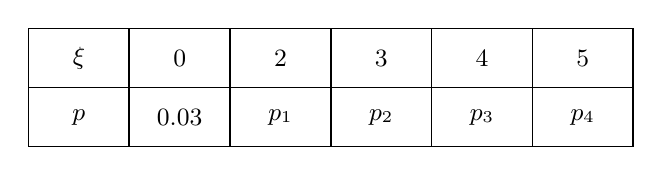
\begin{tikzpicture}[scale=1.0, semithick, every node/.style={inner sep=3.5pt, font=\small}]
  \draw (0,0) rectangle (7.68,-1.5);
  \draw (0,-0.75) -- (7.68,-0.75);
  \foreach \x in {1.28, 2.56, 3.84, 5.12, 6.4} {
    \draw (\x,0) -- (\x,-1.5);
  }
  \node at (0.64,-0.375) {$\xi$};
  \node at (1.92,-0.375) {$0$};
  \node at (3.2,-0.375) {$2$};
  \node at (4.48,-0.375) {$3$};
  \node at (5.76,-0.375) {$4$};
  \node at (7.04,-0.375) {$5$};
  \node at (0.64,-1.125) {$p$};
  \node at (1.92,-1.125) {$0.03$};
  \node at (3.2,-1.125) {$p_1$};
  \node at (4.48,-1.125) {$p_2$};
  \node at (5.76,-1.125) {$p_3$};
  \node at (7.04,-1.125) {$p_4$};
\end{tikzpicture}
\end{center}
\nopagebreak[4]
（1）求 $q_2$ 的值；

（2）求随机变量 $\xi$ 的数学期望 $E\xi$；

（3）试比较该同学选择都在 $B$ 处投篮得分超过 $3$ 分与选择上述方式投篮得分超过 $3$ 分的概率的大小．

\Needspace{4\baselineskip}
\textbf{解析}

\Needspace{5\baselineskip}
（1）$\xi=0$ 表示三次投篮都没进：

\nopagebreak[4]
\[P(\xi=0)=(1-q_1)(1-q_2)^2=0.03 .\]

由 $1-q_1=0.75$ 得 $(1-q_2)^2=0.04$，故 $q_2=0.8$。

（2）各取值的概率：

\begin{itemize}
\item $\xi=0$：$0.75\times0.2^2=0.03$；
\item $\xi=2$：$0.75\times2\times0.8\times0.2=0.24$；
\item $\xi=3$：$0.25\times0.2^2=0.01$；
\item $\xi=4$：$0.75\times0.8^2=0.48$；
\item $\xi=5$：$0.25\times0.8+0.25\times0.2\times0.8=0.24$。
\end{itemize}

\nopagebreak[4]
\[E\xi=0\cdot0.03+2\cdot0.24+3\cdot0.01+4\cdot0.48+5\cdot0.24=3.63 .\]

\Needspace{5\baselineskip}
（3）按「先 $A$ 后 $B$」的方式：

\nopagebreak[4]
\[P(\xi>3)=P(\xi=4)+P(\xi=5)=0.48+0.24=0.72 .\]

\Needspace{5\baselineskip}
若三次都在 $B$ 处投，得分超过 $3$ 分即至少投进两球：

\nopagebreak[4]
\[P=0.8^3+\mathrm C_3^2\cdot0.8^2\cdot0.2=0.512+0.384=0.896 .\]

因 $0.896>0.72$，都在 $B$ 处投篮时得分超过 $3$ 分的概率更大。

\gkanswer{答案：（1）$q_2=0.8$；（2）$E\xi=3.63$；（3）都在 $B$ 处投的得分超过 $3$ 分的概率更大。}

\end{answer}
\begin{answer}
\gksolhead{20}{}

\textbf{题目}：

等比数列 $\{a_n\}$ 的前 $n$ 项和为 $S_n$．已知对任意的 $n\in\mathbf N^*$，点 $(n,S_n)$ 均在函数 $y=b^x+r$（$b>0$ 且 $b\neq1$，$b,r$ 为常数）的图象上．

（1）求 $r$ 的值；

\Needspace{5\baselineskip}
（2）当 $b=2$ 时，记 $b_n=2(\log_2a_n+1)$（$n\in\mathbf N^*$）．证明：对任意的 $n\in\mathbf N^*$，不等式

\nopagebreak[4]
\[\frac{b_1+1}{b_1}\cdot\frac{b_2+1}{b_2}\cdot\ldots\cdot\frac{b_n+1}{b_n}>\sqrt{n+1}\]

成立．

\Needspace{4\baselineskip}
\textbf{解析}

\Needspace{5\baselineskip}
（1）$n\geqslant2$ 时

\nopagebreak[4]
\[a_n=S_n-S_{n-1}=(b-1)b^{n-1},\]

\Needspace{5\baselineskip}
$n=1$ 时 $a_1=S_1=b+r$。等比数列要求

\nopagebreak[4]
\[a_1=\frac{a_2}{b}=b-1\ \Longrightarrow\ r=-1 .\]

\Needspace{5\baselineskip}
（2）$b=2$ 时 $a_n=2^{n-1}$，

\nopagebreak[4]
\[b_n=2(\log_2a_n+1)=2(n-1+1)=2n .\]

\Needspace{5\baselineskip}
待证

\nopagebreak[4]
\[\prod_{k=1}^{n}\frac{2k+1}{2k}>\sqrt{n+1}.\]

\Needspace{5\baselineskip}
$n=1$ 时 $\frac32>\sqrt2$ 成立。设 $n$ 时成立，则

\nopagebreak[4]
\[\prod_{k=1}^{n+1}\frac{2k+1}{2k}>\sqrt{n+1}\cdot\frac{2n+3}{2n+2}.\]

\Needspace{5\baselineskip}
只需证

\nopagebreak[4]
\[\sqrt{n+1}\cdot\frac{2n+3}{2n+2}>\sqrt{n+2}
\iff (n+1)(2n+3)^2>(n+2)(2n+2)^2 .\]

左边 $=4n^3+16n^2+21n+9$，右边 $=4n^3+16n^2+20n+8$，差为 $n+1>0$，故成立。

由数学归纳法，对一切 $n\in\mathbf N^*$ 不等式成立。

\gkanswer{答案：（1）$r=-1$；（2）证明见解析。}

\end{answer}
\begin{answer}
\gksolhead{21}{}

\textbf{题目}：

两县城 $A$ 和 $B$ 相距 $20\ \mathrm{km}$，现计划在两县城外以 $AB$ 为直径的半圆弧 $\overset{\frown}{AB}$ 上选择一点 $C$ 建造垃圾处理厂，其对城市的影响度与所选地点到城市的距离有关，对城 $A$ 和城 $B$ 的总影响度为城 $A$ 与城 $B$ 的影响度之和．记 $C$ 点到城 $A$ 的距离为 $x\ \mathrm{km}$，建在 $C$ 处的垃圾处理厂对城 $A$ 和城 $B$ 的总影响度为 $y$．统计调查表明：垃圾处理厂对城 $A$ 的影响度与所选地点到城 $A$ 的距离的平方成反比，比例系数为 $4$；对城 $B$ 的影响度与所选地点到城 $B$ 的距离的平方成反比，比例系数为 $k$．当垃圾处理厂建在 $\overset{\frown}{AB}$ 的中点时，对城 $A$ 和城 $B$ 的总影响度为 $0.065$．

（1）将 $y$ 表示成 $x$ 的函数；

（2）讨论（1）中函数的单调性，并判断弧 $\overset{\frown}{AB}$ 上是否存在一点，使建在此处的垃圾处理厂对城 $A$ 和城 $B$ 的总影响度最小？若存在，求出该点到城 $A$ 的距离；若不存在，说明理由．

\Needspace{4\baselineskip}
\textbf{解析}

\Needspace{5\baselineskip}
（1）因 $AB$ 为圆的直径，$\angle ACB=90^\circ$，故

\nopagebreak[4]
\[BC^2=AB^2-AC^2=400-x^2 .\]

\Needspace{5\baselineskip}
于是

\nopagebreak[4]
\[y=\frac{4}{x^2}+\frac{k}{400-x^2}\qquad(0<x<20).\]

\Needspace{5\baselineskip}
当 $C$ 为弧 $AB$ 的中点时 $AC=BC=10\sqrt2$，

\nopagebreak[4]
\[\frac{4}{200}+\frac{k}{200}=0.065\ \Longrightarrow\ 4+k=13\ \Longrightarrow\ k=9 .\]

\Needspace{5\baselineskip}
故

\nopagebreak[4]
\[y=\frac{4}{x^2}+\frac{9}{400-x^2}\qquad(0<x<20).\]

\Needspace{5\baselineskip}
（2）

\nopagebreak[4]
\[y'=-\frac{8}{x^3}+\frac{18x}{(400-x^2)^2}.\]

\Needspace{5\baselineskip}
令 $y'=0$：

\nopagebreak[4]
\[18x^4=8(400-x^2)^2\ \Longrightarrow\ 9x^4=4(400-x^2)^2\ \Longrightarrow\ 3x^2=2(400-x^2),\]

\nopagebreak[4]
\[5x^2=800\ \Longrightarrow\ x^2=160\ \Longrightarrow\ x=4\sqrt{10}.\]

当 $0<x<4\sqrt{10}$ 时 $y'<0$，$y$ 递减；当 $4\sqrt{10}<x<20$ 时 $y'>0$，$y$ 递增。故 $x=4\sqrt{10}$ 时 $y$ 取最小值，即弧上存在这样的点，它到城 $A$ 的距离为 $4\sqrt{10}\ \mathrm{km}$。

\gkanswer{答案：（1）$y=\dfrac{4}{x^2}+\dfrac{9}{400-x^2}$（$0<x<20$）；（2）存在，该点到城 $A$ 的距离为 $4\sqrt{10}\ \mathrm{km}$。}

\end{answer}
\begin{answer}
\gksolhead{22}{}

\textbf{题目}：

设椭圆 $E:\dfrac{x^2}{a^2}+\dfrac{y^2}{b^2}=1$（$a>b>0$）过 $M(2,\sqrt2)$，$N(\sqrt6,1)$ 两点，$O$ 为坐标原点．

（1）求椭圆 $E$ 的方程；

（2）是否存在圆心在原点的圆，使得该圆的任意一条切线与椭圆 $E$ 恒有两个交点 $A,B$，且 $\overrightarrow{OA}\perp\overrightarrow{OB}$？若存在，写出该圆的方程，并求 $|AB|$ 的取值范围；若不存在，说明理由．

\Needspace{4\baselineskip}
\textbf{解析}

\Needspace{5\baselineskip}
（1）代入两点：

\nopagebreak[4]
\[\frac{4}{a^2}+\frac{2}{b^2}=1,\qquad \frac{6}{a^2}+\frac{1}{b^2}=1 .\]

\Needspace{5\baselineskip}
相减得 $\dfrac{2}{a^2}=\dfrac{1}{b^2}$，即 $a^2=2b^2$。代回第一式：

\nopagebreak[4]
\[\frac{4}{2b^2}+\frac{2}{b^2}=\frac{4}{b^2}=1\ \Longrightarrow\ b^2=4,\quad a^2=8 .\]

\Needspace{5\baselineskip}
故

\nopagebreak[4]
\[E:\ \frac{x^2}{8}+\frac{y^2}{4}=1 .\]

\Needspace{5\baselineskip}
（2）设圆 $x^2+y^2=r^2$，其切线 $y=kx+t$ 满足

\nopagebreak[4]
\[\frac{|t|}{\sqrt{1+k^2}}=r\ \Longrightarrow\ t^2=r^2(1+k^2).\]

\Needspace{5\baselineskip}
代入椭圆并乘以 $8$：

\nopagebreak[4]
\[x^2(1+2k^2)+4ktx+2t^2-8=0 .\]

\Needspace{5\baselineskip}
设 $A(x_1,y_1)$、$B(x_2,y_2)$：

\nopagebreak[4]
\[x_1+x_2=-\frac{4kt}{1+2k^2},\qquad x_1x_2=\frac{2t^2-8}{1+2k^2}.\]

\nopagebreak[4]
\[\overrightarrow{OA}\cdot\overrightarrow{OB}
=(1+k^2)x_1x_2+kt(x_1+x_2)+t^2 .\]

\Needspace{5\baselineskip}
通分后分子为

\nopagebreak[4]
\[(1+k^2)(2t^2-8)-4k^2t^2+t^2(1+2k^2)=3t^2-8(1+k^2),\]

\Needspace{5\baselineskip}
故

\nopagebreak[4]
\[\overrightarrow{OA}\cdot\overrightarrow{OB}=\frac{3t^2-8(1+k^2)}{1+2k^2}.\]

\Needspace{5\baselineskip}
故

\nopagebreak[4]
\[\overrightarrow{OA}\perp\overrightarrow{OB}\iff 3t^2=8(1+k^2)\iff r^2=\frac83 .\]

\Needspace{5\baselineskip}
竖直切线 $x=\pm\dfrac{2\sqrt6}{3}$ 单独验证：以 $x^2=\dfrac83$ 代入椭圆得 $y^2=\dfrac83$，两交点关于 $x$ 轴对称，

\nopagebreak[4]
\[\overrightarrow{OA}\cdot\overrightarrow{OB}=x^2-y^2=0 .\]

\Needspace{5\baselineskip}
故存在圆

\nopagebreak[4]
\[x^2+y^2=\frac83 .\]

\Needspace{5\baselineskip}
求 $|AB|$：设 $u=k^2\geqslant0$，由 $t^2=\dfrac83(1+k^2)$，

\nopagebreak[4]
\[(x_1-x_2)^2=(x_1+x_2)^2-4x_1x_2
=\frac{32(4u+1)}{3(1+2u)^2},\]

\nopagebreak[4]
\[|AB|^2=(1+u)(x_1-x_2)^2=\frac{32}{3}\cdot\frac{(1+u)(4u+1)}{(1+2u)^2}.\]

\Needspace{5\baselineskip}
记

\nopagebreak[4]
\[g(u)=\frac{(1+u)(4u+1)}{(1+2u)^2},\]

\nopagebreak[4]
\[g'(u)=\frac{(8u+5)(1+2u)^2-4(4u^2+5u+1)(1+2u)}{(1+2u)^4}
=\frac{1-4u^2}{(1+2u)^3},\]

\Needspace{5\baselineskip}
故 $g$ 在 $u=\dfrac12$ 处取最大值 $g\left(\dfrac12\right)=\dfrac98$。又

\nopagebreak[4]
\[|AB|^2\Big|_{u=0}=\frac{32}{3},\qquad |AB|^2\Big|_{u=1/2}=12,\qquad \lim_{u\to+\infty}|AB|^2=\frac{32}{3},\]

\Needspace{5\baselineskip}
故

\nopagebreak[4]
\[|AB|^2\in\left[\frac{32}{3},12\right],\qquad |AB|\in\left[\frac{4\sqrt6}{3},2\sqrt3\right].\]

\gkanswer{答案：（1）$\dfrac{x^2}{8}+\dfrac{y^2}{4}=1$；（2）存在，圆 $x^2+y^2=\dfrac83$，$|AB|\in\left[\dfrac{4\sqrt6}{3},2\sqrt3\right]$。}

\end{answer}